\section{Exceptional Control Flow}

\begin{concept}{Exception Types}
Two main categories of exceptions:

\textbf{Interrupt Sources:}
\begin{itemize}
  \item Peripherals signal to CPU that an event needs immediate attention
  \item Can alternatively be generated by software request
  \item Asynchronous to instruction execution
\end{itemize}

\textbf{System Exceptions:}
\begin{itemize}
  \item \textbf{Reset}: Processor restart
  \item \textbf{NMI}: Non-maskable Interrupt (cannot be ignored)
  \item \textbf{Faults}: Undefined instructions, errors
  \item \textbf{System Calls}: OS calls - Instructions SVC and PendSV
\end{itemize}
\end{concept}

\begin{definition}{Interrupt Control}\\
PRIMASK register controls interrupt handling:
\begin{itemize}
  \item Single bit controls all maskable interrupts
  \item Reset state: PRIMASK = 0 (interrupts enabled)
  \item Control methods:
    \begin{itemize}
      \item Assembly: \texttt{CPSID i} (disable), \texttt{CPSIE i} (enable)
      \item C: \texttt{\_\_disable\_irq()}, \texttt{\_\_enable\_irq()}
    \end{itemize}
\end{itemize}

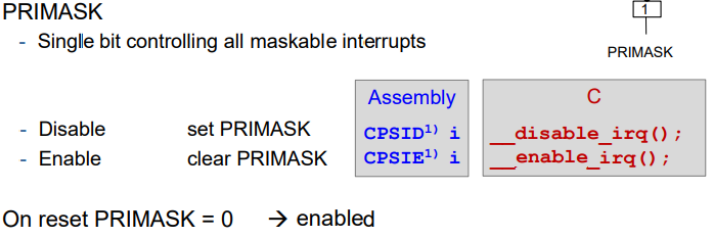
\includegraphics[width=\linewidth]{images/primask.png}
\end{definition}

\begin{definition}{Context Storage}
Interrupt handling requires automatic context saving

\textbf{Timing:} Interrupts can occur at any time (e.g. between instructions)
\begin{itemize}
  \item CPU must save current state before handling
  \item Context includes registers, flags, and program counter
\end{itemize}

\textbf{ISR call:}
\begin{itemize}
  \item requires automatic save off lags and caller saved registers
  \item Stores on stack:
    \begin{itemize}
      \item xPSR, PC, LR, R12
      \item R0-R3 (caller-saved registers)
    \end{itemize}
  \item Stores EXC\_RETURN in LR
\end{itemize}

\textbf{ISR return:}
\begin{itemize}
  \item Use BX LR or POP {..., PC}
  \item Loading EXC return into PC $\rightarrow$ restores from stack:
    \begin{itemize}
      \item R0-R3, R12, LR, PC, xPSR
    \end{itemize}
\end{itemize}
\end{definition}

\begin{example2}{Basic ISR Implementation}
\begin{lstlisting}[language=armasm, style=basesmol]
    ; Interrupt Service Routine
    EXPORT MyISR
MyISR
    PUSH    {R4-R7, LR}    ; Save registers
    
    ; Handle interrupt here
    ; R0-R3 already saved automatically
    
    POP     {R4-R7, PC}    ; Restore and return
\end{lstlisting}
\end{example2}

\subsubsection{Interrupt Handling}

\begin{corollary}{Interrupt Basics}\\
Key concepts for interrupt handling:
\begin{itemize}
  \item \textbf{Interrupt Sources}:
    \begin{itemize}
      \item Hardware interrupts from peripherals
      \item Software interrupts (SVC)
      \item System exceptions
    \end{itemize}
  \item \textbf{Configuration Steps}:
    \begin{itemize}
      \item Enable specific interrupt source
      \item Install interrupt handler
      \item Configure interrupt priority
      \item Enable global interrupts
    \end{itemize}
  \item \textbf{Handler Requirements}:
    \begin{itemize}
      \item Predefined names from vector table
      \item No return values allowed
      \item Must clear interrupt flags
      \item Save/restore used registers
    \end{itemize}
\end{itemize}
\end{corollary}

\begin{concept}{Interrupt-Driven I/O}
\begin{itemize}
  \item Hardware-triggered event handling
  \item Asynchronous to main program
\end{itemize}

\textbf{Main program:}
    \begin{itemize}
      \item Initializes peripherals, afterwards executes other tasks
      \item Peripherals signal when they require SW attention
      \item Events interrupt program execution
    \end{itemize}

\begin{minipage}{0.6\linewidth}
\begin{itemize}
  \item \textbf{Advantages:}
    \begin{itemize}
      \item Efficient CPU usage\\ (no busy waiting)
      \item Quick response times
      \item Better system throughput
    \end{itemize}
  \item \textbf{Disadvantages:}
    \begin{itemize}
      \item No synchronization between \\main program and ISR %TODO: is this correct?
      \item More complex implementation \\ and harder to debug
      \item Timing less predictable
    \end{itemize}
\end{itemize}
\end{minipage}
\begin{minipage}{0.39\linewidth}
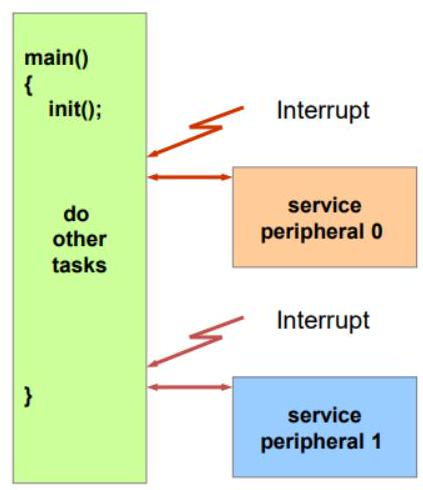
\includegraphics[width=\linewidth]{images/2024_12_29_79e6b22f503fb7b4f718g-11(2)}
\end{minipage}
\end{concept}

\begin{concept}{Polling} Periodic query of status information

  \textbf{Main program:}
    \begin{itemize}
      \item Reading of status registers in loop
      \item Continues execution if no event
      \item Handles event if detected
      \item Synchronous with main program
    \end{itemize}

  \begin{minipage}{0.6\linewidth}
\begin{itemize}
  \item \textbf{Advantages:}
    \begin{itemize}
      \item Simple and straightforward
      \item Implicit synchronization
      \item Predictable timing (deterministic)
      \item No additional interrupt \\logic required
    \end{itemize}
  \item \textbf{Disadvantages:}
    \begin{itemize}
      \item CPU wastes time waiting (busy wait)
      \item Reduced system throughput
      \item Longer response times
    \end{itemize}
\end{itemize}
\end{minipage}
\begin{minipage}{0.39\linewidth}
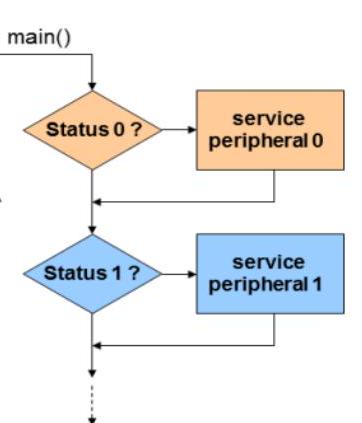
\includegraphics[width=\linewidth]{images/2024_12_29_79e6b22f503fb7b4f718g-11(1)}
\end{minipage}
\end{concept}





\begin{formula}{Interrupt Control}

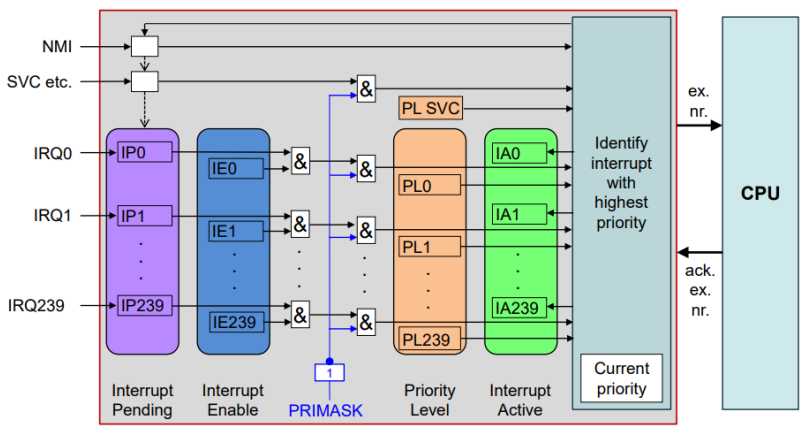
\includegraphics[width=\linewidth]{images/interrupt_control.png}
\end{formula}


\begin{definition}{Program Status Registers (PSR)}
  \begin{itemize}
    \item \textbf{IPSR}: Interrupt Program Status Register
    \item \textbf{EPSR}: Execution Program Status Register
    \item \textbf{APSR}: Application Program Status Register
    \item \textbf{xPSR}: Extended Program Status Register (combination of all three above)
  \end{itemize}
  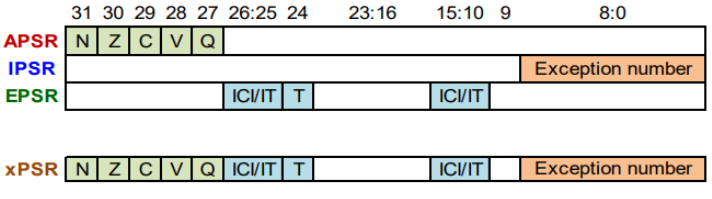
\includegraphics[width=\linewidth]{images/psrs.png}
\end{definition}

\begin{concept}{Priority System}
Interrupt priority handling:
\begin{itemize}
  \item \textbf{Priority Levels}:
    \begin{itemize}
      \item 0-255 (lower number = higher priority)
      \item Fixed priorities for system exceptions
      \item Programmable priorities for IRQs
    \end{itemize}
  \item \textbf{Preemption}:
    \begin{itemize}
      \item Higher priority interrupts can preempt lower
      \item Same priority follows FIFO
    \end{itemize}
\end{itemize}
\end{concept}

\begin{definition}{Nested Exceptions}\\
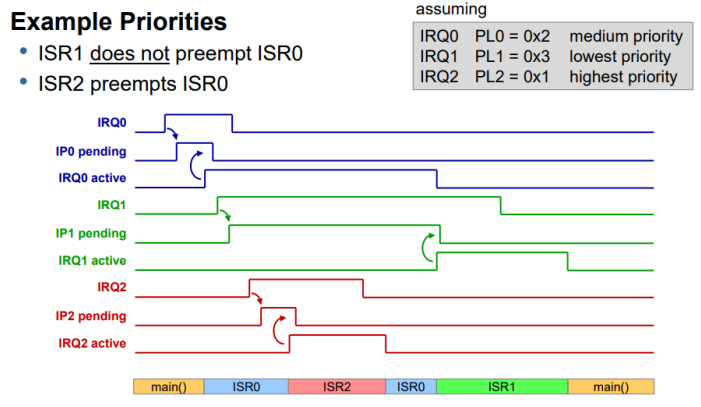
\includegraphics[width=\linewidth]{images/nested_exceptions.png}  
\end{definition}

\subsubsection{Nested Vectored Interrupt Controller (NVIC)}

\begin{concept}{NVIC (Nested Vectored Interrupt Controller)}\\
\textbf{Interrupt/Exception States}:
    \begin{itemize}
      \item \textbf{Inactive}: Not active and not pending
      \item \textbf{Pending}: Waiting to be serviced by CPU
      or: Interrupt event occurred (IRQn=1), but interrupts are disabled (PRIMASK=1)
      \item \textbf{Active}: Currently being serviced by CPU but not yet completed
      \item \textbf{Active and Pending}: \\Being serviced with new request pending for same source
    \end{itemize}
\textbf{Control Registers}:

\begin{minipage}{0.5\linewidth}
    \begin{itemize}
      \item Interrupt Enable (IE)
      \item Interrupt Pending (IP)
    \end{itemize}
\end{minipage}
\begin{minipage}{0.49\linewidth}
    \begin{itemize}
      \item Interrupt Active (IA)
      \item Priority Level (PL)
    \end{itemize}
\end{minipage}
\end{concept}



\begin{formula}{Interrupt Control Registers}
Important NVIC registers:

1. Enable/Disable Registers:
\begin{lstlisting}[language=armasm, style=basesmol]
SETENA0 EQU 0xE000E100    ; Enable interrupts
CLRENA0 EQU 0xE000E180    ; Disable interrupts
; Enable IRQ3
LDR     R0, =SETENA0
MOVS    R1, #(1<<3)
STR     R1, [R0]
; Disable IRQ3
LDR     R0, =CLRENA0
MOVS    R1, #(1<<3)
STR     R1, [R0]
\end{lstlisting}

2. Pending Registers:
\begin{lstlisting}[language=armasm, style=basesmol]
SETPEND0 EQU 0xE000E200   ; Set pending
CLRPEND0 EQU 0xE000E280   ; Clear pending
; Set IRQ3 pending
LDR     R0, =SETPEND0
MOVS    R1, #(1<<3)
STR     R1, [R0]
; Clear IRQ3 pending
LDR     R0, =CLRPEND0
MOVS    R1, #(1<<3)
STR     R1, [R0]
\end{lstlisting}
\end{formula}

\begin{KR}{Exception Vector Table}
Setup and usage:

Vector table structure and Handler implementation:
\begin{lstlisting}[language=armasm, style=basesmol]
    AREA RESET, DATA, READONLY
__Vectors
    DCD     __initial_sp        ; Top of Stack
    DCD     Reset_Handler       ; Reset
    DCD     NMI_Handler        ; NMI
    DCD     HardFault_Handler  ; Hard Fault
    DCD     0                  ; Reserved
    DCD     0                  ; Reserved
    ; ... more vectors
    DCD     IRQ0_Handler       ; IRQ0
    DCD     IRQ1_Handler       ; IRQ1
\end{lstlisting}
\vspace{-2mm}
\begin{lstlisting}[language=armasm, style=basesmol]
    AREA |.text|, CODE, READONLY
    
IRQ0_Handler PROC
    EXPORT IRQ0_Handler
    PUSH    {R4-R7,LR}
    ; Handle interrupt
    POP     {R4-R7,PC}
    ENDP
\end{lstlisting}
\end{KR}

\begin{example2}{NVIC Configuration}\\
Complete interrupt system setup:

\begin{lstlisting}[language=C, style=basesmol]
void init_timer_interrupt(void) {
    // Configure timer peripheral
    TIM2->PSC = 7199;        // Prescaler
    TIM2->ARR = 9999;        // Auto-reload value
    TIM2->DIER |= 1;         // Enable interrupt
    TIM2->CR1 |= 1;          // Enable timer
    
    // Configure NVIC
    NVIC_SetPriority(TIM2_IRQn, 2);  // Set priority
    NVIC_EnableIRQ(TIM2_IRQn);       // Enable IRQ
    
    __enable_irq();          // Enable global interrupts
}

// Timer 2 interrupt handler
void TIM2_IRQHandler(void) {
    if (TIM2->SR & 1) {      // Check update flag
        // Handle interrupt
        TIM2->SR &= ~1;      // Clear flag
    }
}
\end{lstlisting}

Assembly equivalent:
\begin{lstlisting}[language=armasm, style=basesmol]
TIM2_BASE    EQU     0x40000000
TIM_SR       EQU     0x10
TIM_DIER     EQU     0x0C
SETENA0      EQU     0xE000E100

    ; Enable timer interrupt
    LDR     R0, =TIM2_BASE
    LDR     R1, [R0, #TIM_DIER]
    ORRS    R1, #1
    STR     R1, [R0, #TIM_DIER]
    
    ; Enable in NVIC
    LDR     R0, =SETENA0
    MOVS    R1, #1
    LSLS    R1, #28         ; IRQ28
    STR     R1, [R0]
\end{lstlisting}
\end{example2}

\begin{remark}
Important considerations:
\begin{itemize}
  \item Always clear interrupt flags
  \item Minimize time in interrupt handlers
  \item Protect shared data access
  \item Consider interrupt priorities
  \item Avoid deadlocks with nested interrupts
\end{itemize}
\end{remark}

\columnbreak

\subsubsection{Data Consistency}

\begin{concept}{Data Consistency}
Handling shared data access:
\begin{itemize}
  \item \textbf{Race Conditions}:
    \begin{itemize}
      \item Main program and ISR accessing same data
      \item Interrupts during multi-step operations
    \end{itemize}
  \item \textbf{Solutions}:
    \begin{itemize}
      \item Disable interrupts during critical sections
      \item Use atomic operations
      \item Implement proper synchronization
    \end{itemize}
\end{itemize}
\end{concept}

\begin{example2}{Data Consistency Protection}\\
Protecting shared data access:

\begin{lstlisting}[language=C, style=basesmol]
// Global time counters accessed by ISR
volatile uint32_t minutes = 0;
volatile uint32_t hours = 0;

// Timer ISR updates counters
void TIM2_IRQHandler(void) {
    minutes++;
    if (minutes >= 60) {
        minutes = 0;
        hours++;
    }
    // Clear interrupt flag
}

// Main code reading counters
void read_time(uint32_t *min, uint32_t *hr) {
    // Disable interrupts to read consistent values
    __disable_irq();
    *min = minutes;
    *hr = hours;
    __enable_irq();
}
\end{lstlisting}

Assembly equivalent:
\begin{lstlisting}[language=armasm, style=basesmol]
read_time
    PUSH    {R4-R5, LR}
    CPSID   i               ; Disable interrupts
    
    LDR     R4, =minutes    ; Load minutes
    LDR     R2, [R4]
    STR     R2, [R0]        ; Store to output
    
    LDR     R5, =hours      ; Load hours
    LDR     R3, [R5]
    STR     R3, [R1]        ; Store to output
    
    CPSIE   i               ; Enable interrupts
    POP     {R4-R5, PC}
\end{lstlisting}
\end{example2}

\columnbreak

\subsubsection{Implementing Interrupt Handlers}

\begin{KR}{Implementing Interrupt Handlers}

\begin{minipage}{0.5\linewidth}
\begin{enumerate}
  \item Define interrupt vector
  \item Save necessary context
  \item Handle the interrupt
  \item Clear interrupt flag
  \item Restore context
  \item Return from interrupt
\end{enumerate}
\end{minipage}
\begin{minipage}{0.49\linewidth}
Important considerations:
\begin{itemize}
  \item Keep ISRs short
  \item Handle critical tasks only
  \item Be aware of nested interrupts
  \item Protect shared resources
\end{itemize}
\end{minipage}
\end{KR}

\begin{KR}{Interrupt Handler Implementation}\\
Guidelines for implementing interrupt handlers:

1. Handler structure:
\begin{lstlisting}[language=armasm, style=basesmol]
handler_name
    PUSH    {R4-R6}          ; Save used registers
    
    ; Check interrupt flags
    ; Handle interrupt condition
    ; Clear interrupt flags
    
    POP     {R4-R6}          ; Restore registers
    BX      LR               ; Return from handler
\end{lstlisting}

2. Register preservation:
\begin{itemize}
  \item R0-R3: Automatically saved by hardware
  \item R4-R11: Must be preserved if used
  \item R12: Can be used freely
  \item LR: Contains special EXC\_RETURN value
\end{itemize}

3. Critical section handling:
\begin{lstlisting}[language=armasm, style=basesmol]
    ; Disable all interrupts
    CPSID   i
    
    ; Critical section code
    ; Access shared resources
    
    ; Enable interrupts
    CPSIE   i
\end{lstlisting}
\end{KR}

\begin{example2}{Timer Interrupt Configuration}
Configuring Timer 2 interrupt:

1. Handler definition:
\begin{lstlisting}[language=armasm, style=basesmol]
    AREA    handlers, CODE, READONLY
    
    EXPORT  TIM2_IRQHandler
TIM2_IRQHandler
    PUSH    {R4-R6}          ; Save registers
    ; Handle interrupt
    POP     {R4-R6}          ; Restore registers
    BX      LR               ; Return
\end{lstlisting}

2. Enable interrupt (IRQ28):
\begin{lstlisting}[language=armasm, style=basesmol]
    AREA    startup, CODE, READONLY
    
SETENA0     EQU     0xE000E100  ; Interrupt enable register
    
    ; Enable Timer 2 interrupt
    LDR     R7, =SETENA0
    MOVS    R6, #1           ; Set bit
    LSLS    R6, #28          ; Shift to IRQ28
    STR     R6, [R7]         ; Enable interrupt
\end{lstlisting}
\end{example2}


\columnbreak

\subsubsection{Exception Handling in C}

\begin{KR}{CMSIS Functions for Interrupt Control}\\
Standard CMSIS functions for interrupt handling:
\begin{itemize}
  \item \texttt{NVIC\_EnableIRQ(IRQn)}: Enable specific interrupt
  \item \texttt{NVIC\_DisableIRQ(IRQn)}: Disable specific interrupt
  \item \texttt{NVIC\_SetPendingIRQ(IRQn)}: Set interrupt pending
  \item \texttt{NVIC\_ClearPendingIRQ(IRQn)}: Clear pending status
  \item \texttt{NVIC\_SetPriority(IRQn, priority)}: Set priority
  \item \texttt{NVIC\_GetPriority(IRQn)}: Read priority
\end{itemize}

Example usage:
\begin{lstlisting}[language=C, style=basesmol]
void init_timer_interrupt(void) {
    // Enable timer interrupt
    NVIC_EnableIRQ(TIM2_IRQn);
    
    // Set priority
    NVIC_SetPriority(TIM2_IRQn, 2);
    
    // Configure timer
    // ...
    
    // Enable global interrupts
    __enable_irq();
}
\end{lstlisting}
\end{KR}


\begin{example2}{Data Consistency}
  Example protection:
\begin{lstlisting}[language=C, style=basesmol]
void update_shared_data(void) {
    __disable_irq();         // Critical section start
    shared_var++;           // Update shared data
    __enable_irq();         // Critical section end
}
\end{lstlisting}
\end{example2}

\begin{example2}{Nested Interrupts Example}
Implementation with different priorities:
\begin{lstlisting}[language=C, style=basesmol]
// Initialize interrupts
void init_interrupts(void) {
    // Enable interrupts
    NVIC_EnableIRQ(IRQ0_IRQn);
    NVIC_EnableIRQ(IRQ1_IRQn);
    
    // Set priorities
    NVIC_SetPriority(IRQ0_IRQn, 1); // Higher
    NVIC_SetPriority(IRQ1_IRQn, 2); // Lower
    
    // Enable global interrupts
    __enable_irq();
}

// Higher priority ISR
void IRQ0_Handler(void) {
    // Handle high priority interrupt
    // Can't be interrupted by IRQ1
}

// Lower priority ISR
void IRQ1_Handler(void) {
    // Handle low priority interrupt
    // Can be interrupted by IRQ0
}
\end{lstlisting}
\end{example2}









